%%
%% $Id$
%%
%% Copyright (c) 2007-2008 Christian Fehler
%% Copyright (c) 2007-2008 Benjamin Mies
%%


\chapter{Wie erstelle ich eine neue Grammatik?}\label{Grammar}

Wir wollen das jetzt einmal an Hand folgenden Beispiels aus den
Vorlesungsunterlagen durchgehen:\vspace{10pt}


\begin{tabular}{lcr}
G = ($\Sigma, N, S, P )\ mit $\\
$\Sigma = \{\TerminalSymbol{0}, \TerminalSymbol{1}, \TerminalSymbol{x},
\TerminalSymbol{y}, \TerminalSymbol{-}, \TerminalSymbol{+},
\TerminalSymbol{*}, \TerminalSymbol{(}, \TerminalSymbol{)}\}$\\ $N =
\{\StartSymbol{E}\}$\\ $S=\StartSymbol{E}$\\
$P = \{\StartSymbol{E} \to \TerminalSymbol{0},\ \StartSymbol{E} \to \TerminalSymbol{1},\
\StartSymbol{E}	\to \TerminalSymbol{x},\ \StartSymbol{E} \to \TerminalSymbol{y},\
\StartSymbol{E} \to (\TerminalSymbol{-}\StartSymbol{E}),$\\
$\ \ \ \ \ \ \ \ \StartSymbol{E} \to (\StartSymbol{E} \TerminalSymbol{+}
\StartSymbol{E}),\ \StartSymbol{E} \to (\StartSymbol{E} \TerminalSymbol{-} \StartSymbol{E}),\
\StartSymbol{E} \to (\StartSymbol{E} \TerminalSymbol{*} \StartSymbol{E})\}$\\
\end{tabular}

\section{Neue Grammatik Datei anlegen}

Am Anfang müssen wir dazu erst einmal den "`Neu\ldots"' Dialog öffnen. Zu finden
ist dieser in der Toolbar oder im Menüeintrag "`Datei"'. Dort wählen wir aus,
dass wir eine Grammatik erstellen wollen und klicken auf "`Weiter"'.\vspace{10pt}

Im nächsten Dialog werden wir gefragt, von welchem Typ unsere neue Grammatik
sein soll. In unserem Beispiel handelt es sich um eine "`Kontextfreie
Grammatik"', welche wir auswählen und mit "`Weiter"' bestätigen.\vspace{10pt}

Als nächstes müssen wir die benötigten Nichtterminalzeichen (N),
Terminalzeichen ($\Sigma$) und das Startzeichen (S) angeben.  Als Zeichen
können alle Symbole werwendet werden, die nicht zur Syntax der Eingabe gehören.
Das bedeutet \Symbol{,}, \Symbol{\{}, \Symbol{\}} und \SymbolEmpty{}
können hier nicht verwendet werden. Symbole, welche länger als ein Zeichen sind,
müssen in Anführungszeichen angegeben werden.\vspace{10pt}

In dem Dialog sind an allen Stellen schon vordefinierte Werte eingetragen.
Dabei handelt es sich um die Vorgaben, die man als Standardwerte in den
Einstellungen eingetragen hat.

Wie man diese Standardwerte ändert, kann man in Kapitel \ref{Preferences}
nachlesen. Wir tragen jetzt als erstes die von uns benötigten
Nichtterminalzeichen ein. Dabei handelt es sich bei uns lediglich um das Symbol
\StartSymbol{E}. Also schreiben wir in das Feld
"`\{\StartSymbol{E}\}"'.\vspace{10pt}

Nun legen wir das Startzeichen fest. Das ist bei uns das \StartSymbol{E},
welches wir in das Feld für das Startzeichen schreiben.\\
Zum Schluss müssen wir noch die Terminalzeichen festlegen. Dazu tragen
wir in das entsprechende Feld "`\{\TerminalSymbol{0}, \TerminalSymbol{1},
\TerminalSymbol{x}, \TerminalSymbol{y}, \TerminalSymbol{-}, \TerminalSymbol{+},
\TerminalSymbol{*}, \TerminalSymbol{(}, \TerminalSymbol{)}\}"' ein.\\ Damit
haben wir alle benötigten Information eingegeben und können die neue Grammatik
durch Klick auf "`Fertig"' erstellen.\vspace{10pt}

\begin{figure}[h]
\begin{center}
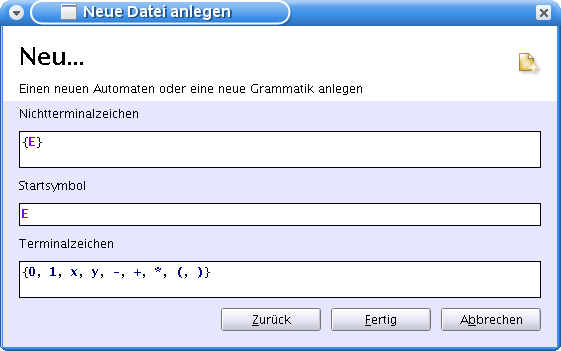
\includegraphics[width=8cm]{../images/new_dialog_grammar.png}
\caption{Grammatik - Neu Dialog}
\end{center}
\end{figure}

Alle Einstellungen, die wir gerade im letzen Dialog für die neue Datei getroffen
haben, lassen sich über "`Dokument editieren"' nachträglich ändern.

\section{Anlegen von Produktionen}

Um eine neue Produktion anzulegen, können wir den entsprechenden Button in der
Toolbar verwenden oder über den Kontextmenüeintrag gehen.\vspace{10pt}

Im Dialog für neue Produktionen müssen wir zunächst einmal angeben, für welches
Nichtterminalzeichen wir eine Produktion anlegen möchten. Dieses können wir aus
einer Liste der verfügbaren Zeichen auswählen. Da wir in unserem Beispiel nur
ein Nichtterminalzeichen haben, ist schon das richtige ausgewählt, und wir
können diesen Schritt überspringen.\vspace{10pt}

Jetzt müssen wir noch das Produktions-Wort angeben. Als Hilfestellung wird in
dem Dialog angezeigt, welche Nichtterminalzeichen und Terminalzeichen uns zur
Verfügung stehen. Wir fangen an mit der Produktion "`$\StartSymbol{E} \to
(\StartSymbol{E} \TerminalSymbol{+} \StartSymbol{E})$"'. Also geben wir als
Produktions Wort "`(\StartSymbol{E} \TerminalSymbol{+} \StartSymbol{E})"' ein.
Als weitere Hilfestellung wird im unteren Dialog die resultierende Produktion im
Ganzen angezeigt. Wir bestätigen den Dialog noch mit "`OK"' und die neue
Produktion erscheint in unserer Liste.\vspace{10pt}

\begin{figure}[h]
\begin{center}
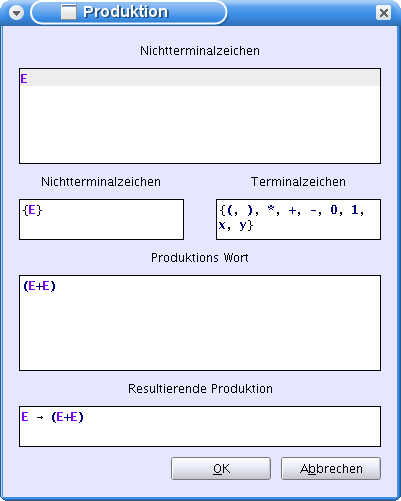
\includegraphics[width=8cm]{../images/production_dialog.png}
\caption{Grammatik - Produktions Dialog}
\end{center}
\end{figure}

Wir können die Produktion selbstverständlich auch editieren und wieder löschen.
Beide Funktionen sind über das Kontextmenü für die ausgewählte Produktion
verfügbar.\vspace{10pt}

Diesen Vorgang wiederholen wir jetzt für unsere komplette Menge "`P"'. Wenn wir
alle Produktionen angelegt haben, sind wir auch mit dem Anlegen der Grammatik
fertig. Es besteht jetzt noch die Möglichkeit, die Grammatik zu validieren, um
zu sehen, ob man beim Erstellen irgendwelche Fehler gemacht hat. Diese Funktion
erreicht man über das Kontextmenü oder über den Menüpunkt "`Ausführen"'.

\begin{figure}[h]
\begin{center}
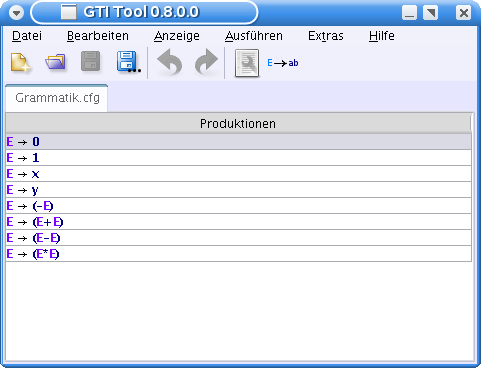
\includegraphics[width=8cm]{../images/cfg_example.png}
\caption{Grammatik - Kontextfreie Grammatik}
\end{center}
\end{figure}

\section{Was fange ich mit einer Grammatik an?}

Wir haben jetzt eine Grammatik angelegt und stellen uns jetzt vielleicht die
Frage, was wir damit eigentlich anfangen können. Es bestehen zur Zeit zwei
Verwendungsmöglichkeiten für eine Grammatik.\vspace{10pt}

Zunächst einmal kann man die Grammatik als Vorlage für eine neue Grammatik
nutzen. Das ist zum Beispiel sinnvoll, wenn wir eine kontextfreie Grammatik
haben und jetzt eine reguläre Grammatik mit den gleichen Produktionen
erstellen wollen. Dazu öffnet man den Menüpunkt "`Ausführen"' und wählt unter
"`Vorlage für\ldots"' den gewünschten Typ der neuen Datei aus.
Dabei ist zu beachten, dass die Grammatik nicht konvertiert wird,
sondern nur als Vorlage verwendet wird.\vspace{10pt}

Die andere Verwendungsmöglichkeit beinhaltet, sich aus der Grammatik einen
ent\-sprechen\-den Automaten generieren zu lassen. Es besteht die Möglichkeit,
sich für eine reguläre Grammatik den entsprechenden NDEA, und für eine
kontextfreie Grammatik den entsprechenden Kellerautomat erzeugen zu
lassen. Zu finden ist die Umwandlung im Menüeintrag "`Ausführen"'
unter "`Umwandeln in\ldots"'.\vspace{10pt}

Es ist zu beachten, dass beim Umwandeln einer Grammatik keine
Validierungsfehler vorhanden sein dürfen. Bei der Funktion "`Vorlage
für\ldots"' spielen Fehler allerdings keine Rolle.

\subsection{Links-Rekursion eliminieren}

Hierzu nutzen wir eine Beispielgrammatik aus der Compilerbau 1-Vorlesung:

\begin{tabular}{lcr}
G = ($\Sigma, N, S, P )\ mit $\\
$\Sigma = \{\TerminalSymbol{a}, \TerminalSymbol{b}, \TerminalSymbol{c},
\TerminalSymbol{d}\}$\\ $N =
\{\NonterminalSymbol{A}, \StartSymbol{S}\}$\\ $S=\StartSymbol{S}$\\
$P = \{\StartSymbol{S} \to \NonterminalSymbol{A}\TerminalSymbol{a},\ \StartSymbol{S} \to \TerminalSymbol{b},\
\NonterminalSymbol{A}	\to \NonterminalSymbol{A}\TerminalSymbol{c},\ \NonterminalSymbol{A} \to \StartSymbol{S}\TerminalSymbol{d},\
\NonterminalSymbol{A} \to \epsilon\}$\\
\end{tabular}

Nun findet man im Menü unter "`Ausführen"' den Punkt "`Links-Rekursion eliminieren"'. Es erscheint das folgende Fenster.

\begin{figure}[h]
\begin{center}
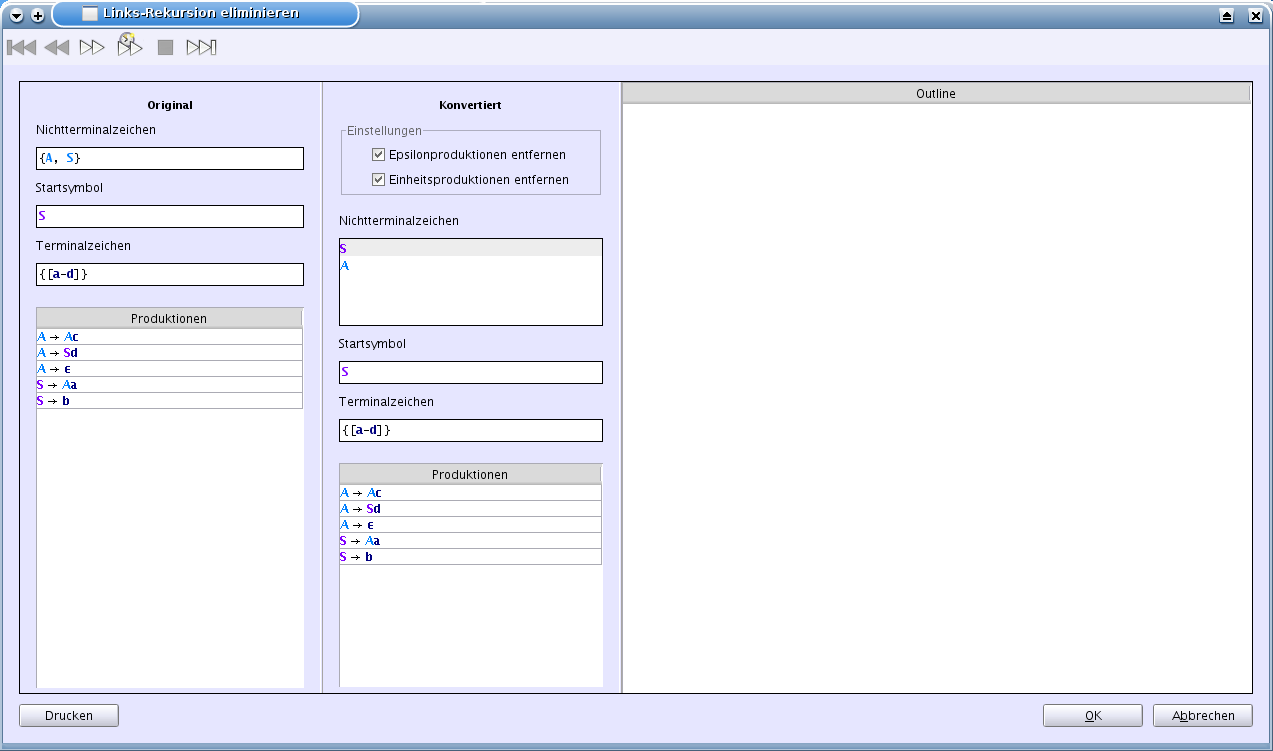
\includegraphics[width=12cm]{../images/left_recursion.png}
\end{center}
\end{figure}

Ganz links befindet sich die ursprüngliche Grammatik. Rechts daneben findet man die neue Grammatik. Diese ist am Anfang gleich der ursprünglichen und wird erst im Verlauf des Algorithmus verändert.

Oben im Fenster der konvertierten Grammatik kann man einstellen, ob zunächst die Epsilon- bzw. Einheitsproduktionen entfernt werden sollen. Diese Möglichkeit wurde gegeben, da der Algorithmus eigentlich eine Grammatik ohne Epsilon- bzw. Einheitsproduktionen verlangt. Aber in dem Beispiel aus der Vorlesung wurde die Epsilonproduktion in der Grammatik belassen mit dem Hinweis, dass dies nichts ausmacht. Da aber das Ergebnis dann nicht exakt das selbe wäre, ist hier die Möglichkeit gegeben, die Produktionen drin zu lassen. Für andere Beispiele sollte man aber diese beiden Optionen an lassen, da sonst der Algorithmus falsche Ergebnisse liefern kann.

In unserem Beispiel schalten wir die Option Epsilonproduktionen entfernen aus.

Als nächstes kann man die Reihenfolge der Nichtterminalzeichen eingestellt werden, da auch diese sich auf die Ergebnisse des Algorithmus auswirken. Die Reihenfolge kann natürlich genau wie die beiden Optionen zum Entfernen von Produktionen nur am Anfang verändert werden.

In der Vorlesung wurde die Reihenfolge $\StartSymbol{S}, \NonterminalSymbol{A}$ gewählt, daher schieben wir das $\NonterminalSymbol{A}$ einfach nach oben.

Nun kann der Algorithmus ablaufen:
\begin{itemize}
  \item Im Initialen Schritt passiert nichts mit der Grammatik, da $i = j$ ist und für $\StartSymbol{S}$ keine direkte Linksrekursion existiert.
  \item Nun kommen durch den Durchlauf im Algorithmus zwei Produktionen ($\NonterminalSymbol{A} \to \NonterminalSymbol{A}\TerminalSymbol{b}\TerminalSymbol{d},\NonterminalSymbol{A} \to \TerminalSymbol{b}\TerminalSymbol{d}$) hinzu und die Produktion $\NonterminalSymbol{A} \to \StartSymbol{S}\TerminalSymbol{d}$ wird entfernt.
  \item Im letzten Schritt dieses Beispiels ist $i = j$ und es wird daher nur noch die direkte Linksrekursion von $\NonterminalSymbol{A}$ entfernt.
\end{itemize}

\subsection{Links-Faktorisierung}

Hierzu nutzen wir eine Beispielgrammatik aus der Compilerbau 1-Vorlesung:

\begin{tabular}{lcr}
G = ($\Sigma, N, S, P )\ mit $\\
$\Sigma = \{\TerminalSymbol{a}, \TerminalSymbol{b}, \TerminalSymbol{e},
\TerminalSymbol{i},\TerminalSymbol{t}\}$\\ $N =
\{\NonterminalSymbol{E}, \StartSymbol{S}\}$\\ $S=\StartSymbol{S}$\\
$P = \{\StartSymbol{S} \to \TerminalSymbol{i}\NonterminalSymbol{E}\TerminalSymbol{t}\StartSymbol{S}\TerminalSymbol{e}\StartSymbol{S},\StartSymbol{S} \to \TerminalSymbol{i}\NonterminalSymbol{E}\TerminalSymbol{t}\StartSymbol{S}, \StartSymbol{S} \to \TerminalSymbol{a}, \NonterminalSymbol{E} \to \TerminalSymbol{b}$\\
\end{tabular}

Nun findet man im Menü unter "`Ausführen"' den Punkt "`Links-Faktorisierung"'. Es erscheint das folgende Fenster.

\begin{figure}[h]
\begin{center}
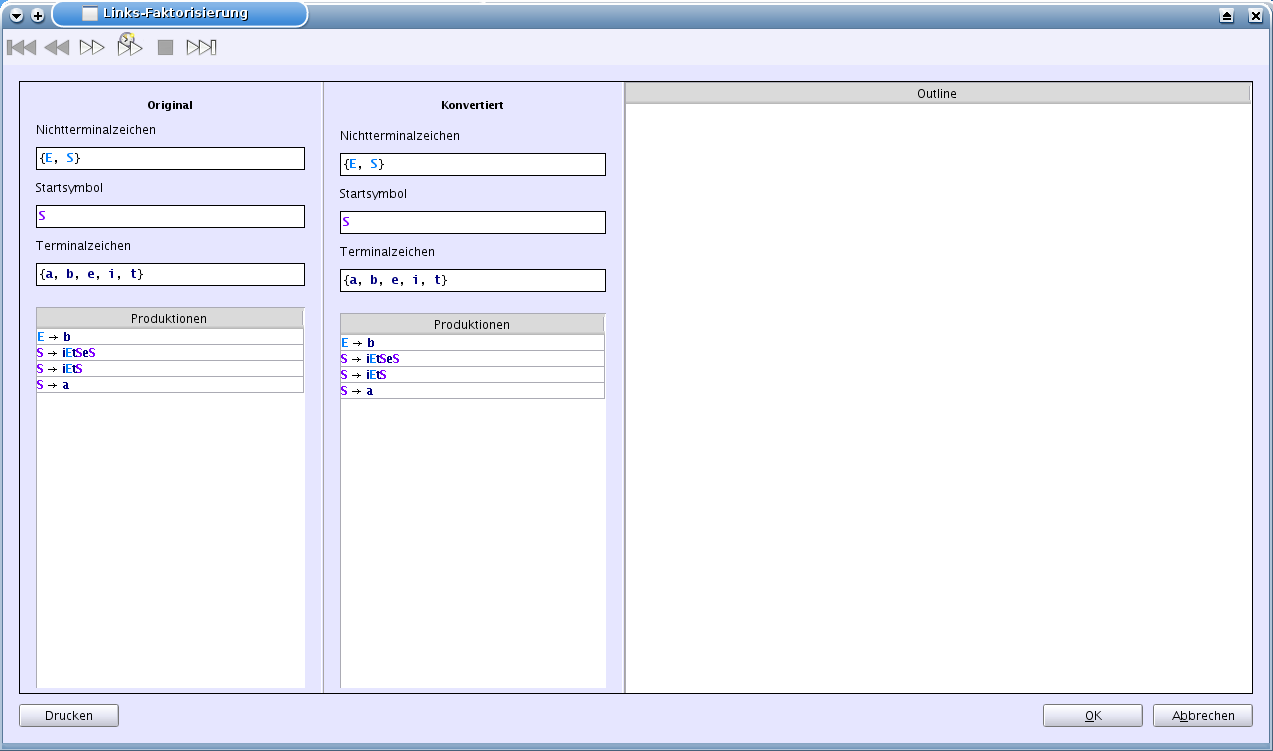
\includegraphics[width=12cm]{../images/left_factoring.png}
\end{center}
\end{figure}

Ganz links befindet sich die ursprüngliche Grammatik. Rechts daneben findet man die konvertierte Grammatik.

Wenn man den Algorithmus dann ablaufen lässt ist der Algorithmus bereits nach einem Schritt fertig. Der Algorithmus findet als längstes gemeinsames Präfix $\TerminalSymbol{i}\NonterminalSymbol{E}\TerminalSymbol{t}\StartSymbol{S}$ und erzeugt ein neues Nichtterminalzeichen $\NonterminalSymbol{S'}$. Als Produktionen kommen hinzu: $\StartSymbol{S} \to \TerminalSymbol{i}\NonterminalSymbol{E}\TerminalSymbol{t}\StartSymbol{S}\NonterminalSymbol{S'}, \NonterminalSymbol{S'} \to \epsilon, \NonterminalSymbol{S'} \to \TerminalSymbol{e}\StartSymbol{S}$, entfernt wurde die Produktion $\StartSymbol{S} \to \TerminalSymbol{i}\NonterminalSymbol{E}\TerminalSymbol{t}\StartSymbol{S}\TerminalSymbol{e}\StartSymbol{S}$.
